\documentclass[conference]{IEEEtran}
% Packages
%\pdfobjcompresslevel=0
\usepackage{titlesec}
\usepackage{graphicx}
\usepackage[style=numeric, backend=biber, sorting=none]{biblatex}
\addbibresource{Communication.bib}
\usepackage{algorithm}
\usepackage{algpseudocode}
\usepackage{booktabs}
\usepackage{float}
\usepackage{multirow}

% Title page
\title{Swarm Dialogues: 
}
\author{Luis Yallico Ylquimiche}
\date{\today}

\begin{document}

% Title page
\maketitle
%add page numbers
\pagestyle{plain}

% Abstract
\begin{abstract}
LOREM IPSUM
\end{abstract}


\section{Introduction}

This study profiles swarm communication on ESP32 hardware, evaluating embodied evolution performance under varied conditions such as agent density, locomotion, topology inference, imposed message budgets and stochastic transmission policies. By focusing on direct peer-to-peer communication links we provide (i) empirical data that probes bottlenecks flagged in recent surveys, and (ii) extract tangible design rules for swarm networks.\\

Swarm engineers draw inspiration from social biological systems such as ants, bees or termites to build decentralised robot collectives that are inherently robust to failure, flexible across tasks and scalable in number \cite{hamann_swarm_2018}. In swarm systems, collective intelligence emerges when individual robots trade packets of information among neighbouring robots. Classic ant-colony-optimisation work in the early 2000s has already proven that an indirect information exchange "virtual-pheromones" can lead to agents collectively discovering optimal routing behaviours \cite{dorigo_ant_2000}. Thus, highlighting the importance of communication design in swarms and the impact it can have over behaviour emergence.\\

While coordination and task allocation have been widely studied in swarm robotics, two recent surveys agree that bandwidth, latency and energy usage are the main blockers to real-world swarm deployments \cite{ding_advancements_2023}\cite{an_multi-robot_2023}. These issues become more pronounced as swarms sizes scale, resulting in an increase in data volumes being transmitted among peers, often overwhelming individual agents' limited compute capabilities. Beyond sheer capacity, the architecture of the communication also matters. Many swarms rely on blind broadcast communication schemes that scale poorly, with collision rates rising sharply beyond a few dozen peers which tend to reduce the reliability of the network \cite{an_multi-robot_2023}.\\

Communication is equally critical when controllers evolve on-line. Recent embodied evolution studies explain that less communication can enhance swarm performance, as trimming neighbourhood size helps populations forget outdated beliefs and re-adapt faster \cite{hiraga_when_2023}\cite{ding_advancements_2023}. Because most of these results stem from simulations,  empirical evidence is still needed to further understand how agent density, throughput and packet content jointly affect evolutionary dynamics and adaptation performance.\\

Viewing communication as a dynamic resource that swarms must actively manage, we present a testing framework that integrates an island-model genetic algorithm (GA) with three distinct communication strategies. These experiments expand our understanding of how communication choices shape embodied evolution performance and supply data needed to tackle the integration challenges outlined above. Accordingly, the following three hypotheses are put forward:\\

\textbf{H1}: Ranking nearby peers by link quality before deciding where to send packets should form a sturdier network with fewer packets being lost.

\textbf{H2}: Even if each robot is allowed to transmit only a fixed number of messages, the group should still reach a common solution over time, the cap is expected to slow premature convergence, not prevent it.

\textbf{H3}: Inserting a brief randomly chosen delay before every transmission should reduce radio collisions and latency, as spreading out broadcasts should address interference in a congested channel.

\section{Related Work}

In \cite{hauert_evolved_2009}, controllers are evolved for ad-hoc aerial relays without positional information, using periodic single-hop broadcasts to neighbours. This concept is leveraged on our experimental setting where the agents exploit link-quality proxies to bias their connections. In non-local communication schemes such as \cite{perrin_decentralised_2012}, network-wide broadcasting is used due to the accelerated diffusion of information, with benefits in search and rescue applications. In contrast, our study uses \emph{unicast} peer-to-peer links at the data-link layer, enabling direct round-trip time measurements.\\

Constrained connectivity repeatedly appears beneficial. The \emph{"less is more"} effect in \cite{talamali_when_2021}, demonstrates that fewer links and lower swarm densities improve adaptation in swarm consensus tasks, by helping robots discard stale beliefs. A similar effect is also observed by \cite{hiraga_when_2023} over embodied evolution, where limiting the genome-exchange range can support the evolutionary search maintain higher diversity for longer and escape local optima. The expectation is that by imposing message quotas and prioritising “distant” islands, the swarm could avoid premature convergence.\\

Transmission timing also matters. Experiments from \cite{aust_hidden_2022} show that limiting the frequency of communication stabilises swarm behavior, while \cite{tsianos_impact_2012} explains that the speed of consensus among peers tolerates random transmission delays even when agents receive multiple out-of-order messages. Furthermore, non-radio data links have also been explored by \cite{trenkwalder_swarmcom_2020}, which shows that infra-red (IR) line-of-sight local communication can be used with benefits such as lower energy requirements per bit and reduced 2.4GHz interference information exchanges albeit with limits on bandwidth and communication range. Complementary work by \cite{rabbah_real_2021} examines real-time, decentralised peer-to-peer middleware at the application layer, addressing IP protocols. It provides a contrast for where to place communication control in swarm systems, whereas we implement this at the MAC layer via ESP-NOW to keep timing and load directly measurable.\\

Over-the-air (OTA) mechanisms tailored to swarms have been explored by \cite{varadharajan_over--air_2018}, where updates are distributed as compact patches using gossip-style communication protocols to ensure version uniformity across large robot groups. We adapt this concept in Section-\ref{sec:ota} to support synchronised firmware across our deployment.\\

%add This is based on the Island model [ref], where different subpopulations (islands) evolve in parallel and occasionally exchange individuals (migration) with other islands, thus enabling the swarm to converge to a solution. 


\section{Experimental Setting}

In this study, a global optimisation problem known as the Rastrigin function Eq. \ref{eq:rastrigin} is used to benchmark the communication performance. This task was chosen to emulate evolutionary controller optimisation, while no controller was actually evolved the concept of robots sending and receiving genomes from their peers remaines the same.\\ 

The environment for the experiments was a rectangular arena without obstacles (Figure \ref{fig:arena}), where the initial positions, and number of the robots was determined by the experiment schedule (Table \ref{tab:exp_config}). All of the experiments were conducted in the same room environment within the department of Engineering Mathematics at the University of Bristol.

\begin{figure}[H]
    \centering
    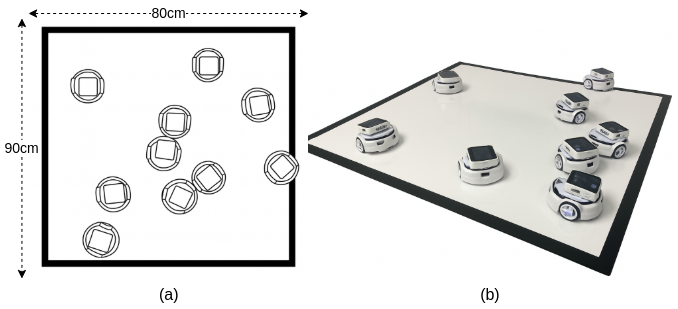
\includegraphics[width=0.49\textwidth]{arena.png}
    \caption{Robot Arena: (a) dimensions and (b) example of a Brownian locomotion experiment with 8 robots.}
    \label{fig:arena}
\end{figure}

Across the study, we evaluated swarm under different communication and system configurations. Each experiment manipulates a specific independent variable while holding all other conditions constant. These include:\\

\begin{itemize}
  \item \textbf{Swarm density}: The number of agents deployed simultaneously, ranging from 3 to 13.
  \item \textbf{Locomotion}: Robots were either \emph{stationary} or navigated using a \emph{Brownian motion} gait (Section \ref{sec:locomotion}).
  \item \textbf{Topology inference}: Transmission priority was governed by either a \emph{stochastic} shuffle or a \emph{comm aware} ranking strategy based on link quality metrics (Section \ref{sec:topology-inference}).
  \item \textbf{Message limits}: A token-bucket rate limiter controlled how frequently agents could transmit messages (Section \ref{sec:limited-rate}).
  \item \textbf{Transmission frequency}: Each message was optionally delayed by a random interval derived from the maximum observed peer latency to reduce potential network collisions (Section \ref{sec:transmission-frequency}).
\end{itemize}

\subsection{Rastrigin Function}

The Rastrigin function is defined as follows:

\begin{equation}\label{eq:rastrigin}
f_R(\mathbf{x}) = 10n + \sum_{i=1}^{n} \left(x_i^2 - 10\cos(2\pi x_i)\right)
\end{equation}

where $n$ is the number of dimensions, in this case the number of genes. Whereas, $x$ is the individual genome being evaluated. The function has a global minimum at \( f_R(\mathbf{x}) = 0 \) when $x = [0, 0, ..., 0]$ for all dimensions \cite{rucinski_impact_2010}. For the purpose of this study we used $n = 10$ and a solution bounded at $-5.12<=x_i<=5.12$.

\subsection{Robot Platform}\label{sec:robot_platform}
\begin{figure}[h]
    \centering
    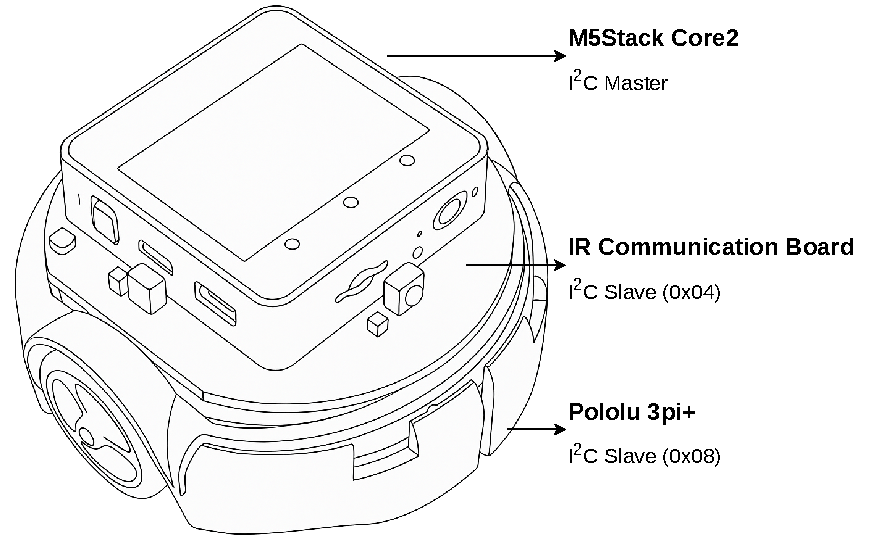
\includegraphics[width=0.45\textwidth]{B2.pdf}
    \caption{The Swarm-B2 platform: M5Stack Core2, IR Communication board, and Pololu 3Pi+}
    \label{fig:B2}
\end{figure}

Table~\ref{tab:B2-hardware} summarises the core hardware components of the Swarm-B2 platform used in this study [REF]. Coordination between devices is handled over a $I^2C$ 100kHz bus. Although the IR board can transmit and receive 32-byte frames, we did not conduct experiments with this feature. The board therefore behaves as a $I^2C$ bridge between the M5 and the Pololu 3Pi+. This guarantees that the communication results in this study stem only from a single data link.\\

\begin{table}[h]
  \centering
  \caption{Swarm-B2 hardware stack}
  \label{tab:B2-hardware}
  \begin{tabular}{p{0.18\linewidth} p{0.22\linewidth} p{0.42\linewidth}}
    \toprule
    Component & Interface(s) & Function \\
    \midrule
    M5Stack Core2 (240 MHz) & $I^2C$ master and SPI & Embodied evolution, ESP-NOW communication, data logging to SD and user interface \\
    IR board (16 MHz) & $I^2C$ slave (0x04) & Bus hub, optional IR feature \\
    Pololu 3Pi+ (16 MHz) & $I^2C$ slave (0x08) & Locomotion, bumper and line following sensors \\

    \bottomrule
  \end{tabular}
\end{table}

The ESP32 was used for running dual-core FreeRTOS parallel tasks, logging data on the local SD card and handling communication via the ESP-NOW data link (2.4 GHz). The 8MB PSRAM and larger flash memory on the master device allowed for concurrent task execution without peripheral starvation.\\

\subsubsection{Locomotion}\label{sec:locomotion}

The Pololu 3Pi+ is equipped with a line following sensor array and two bump sensors, which can be used to detect obstacles and detect the arena edges. A \emph{Brownian-motion} gait was selected to maintain unbiased mobility across the arena and ensure constant movement.\\

The gait code exposes the Pololu 3pi+ slave to the ESP32 master node, this interface lets the ESP32 act as a passenger with override, that can set wheel-speed scaling factors or raise \texttt{START}/\texttt{STOP} flags without touching the low-level control loop. In effect, the Pololu 3pi+ driver handles continuous motion, while the ESP32 decides when to go for each experimental condition.\\

\subsubsection{Local Data Storage}
We implemented local data logging mechanism (Section \ref{sec:data-logging}) on the ESP32 with a 16GB SD card peripheral. The shared SPI bus (with the LCD) was set at a frequency of 20MHz and configured to use the FAT32 file system for storage. This approach was chosen to emulate a realistic swarm system capable of operating remotely without relying on a stable Wi-Fi connection to a central server.\\

\subsubsection{User Interface}

\begin{figure}[h]
    \centering
    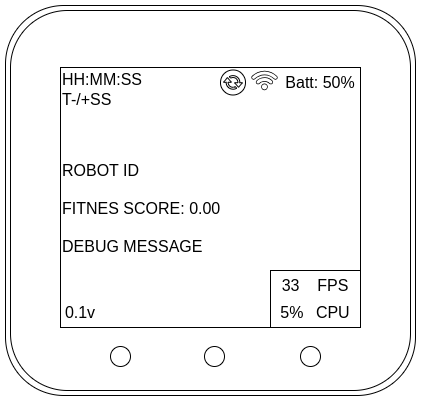
\includegraphics[width=0.35\textwidth]{UI.png}
    \caption{M5 user interface showing the current fitness score and device information.}
    \label{fig:UI}
\end{figure}

Figure \ref{fig:UI} shows the on-board user interface (UI) each Swarm-B2 agent displays during trials. A real-time clock (RTC) seeds a unique \emph{experiment\_id}, just below a $T\pm SS$ counter tells the operator how long until the next minute aligned run. Status lines on the display list the robot's ID (last four hex digits of the MAC address), the live fitness score, and a single debug message. The bottom-left tag logs which software build is running on the device. Two icons round out diagnostics, the Wi-Fi symbol flashes during S3 log upload, and the circular arrow signals an over-the-air update.

\section{Implementation}

This section outlines the software design and implementation of the swarm firmware. The Espressif IoT Development Framework (ESP-IDF) was used as it provides low-level hardware access, offering greater flexibility for ESP-NOW communication (Section \ref{sec:comm-layer}). Unlike the Arduino framework, ESP-IDF provides direct access to FreeRTOS, enabling fine-grained control over concurrent task creation and dual-core processing, such as isolating communication tasks to a specific core. It also supports advanced features like over-the-air (OTA) updates (Section \ref{sec:ota}), unit testing, and custom debugging tools \cite{esp-boards_esp-idf_nodate}.

\subsection{Software Development Environment}\label{sec:SDK}

We employed a Continuous Integration and Continuous Deployment (CI/CD) pipeline via GitHub to automate OTA deployment, ensuring synchronized updates and easier debugging across the swarm (Fig. \ref{fig:cicd-architecture}).\\

The CI/CD integration proved especially valuable during experiments, where consistent updates across multiple agents were necessary. It also facilitated easier rollbacks in the event of unexpected bugs. The automated build pipeline in GitHub ensured that only validated firmware versions were propagated to the swarm, catching any environment discrepancies early in the process.\\

\begin{figure}[h]
    \centering
    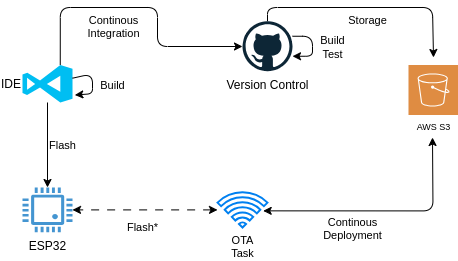
\includegraphics[width=0.45\textwidth]{architecture.png}
    \caption{CI/CD Architecture: Local development, GitHub repository, AWS S3 storage, and OTA updates.}
    \label{fig:cicd-architecture}
\end{figure}

Our software development framework for the swarm is as follows:

\begin{enumerate}
    \item \textbf{Local environment development}: Application development takes place locally using VSCode, our local environment uses version 5.1.4 of ESP-IDF and Python 3.11 to build and flash the code in-situ.\\
    \item \textbf{Version control}: We push updates of the codebase to a public repository on GitHub: \url{https://github.com/yallico/robotics_dissertation}, this allows for version control and triggers a custom build and test process. The ESP32 project is then compiled remotely and generates the binary file used for OTA.\\
    \item \textbf{Cloud storage}: The OTA binary file is uploaded to an AWS S3 public bucket making it accesible to the swarm via HTTPS.\\
\end{enumerate}

\subsubsection{OTA Process}\label{sec:ota}

Upon initialization, each agent checks its local firmware version against the latest version stored in S3. If a mismatch is detected, the ESP32 downloads and installs the updated .bin file. While relying on a central server and exposing the swarm to the internet for updates may seem counterintuitive, a similar update mechanism could be implemented in a decentralized manner using consensus protocols. However, this would have introduced additional complexity beyond the scope of this study.\\

\begin{table}[h]
  \centering
  \caption{System Partition Table}
  \begin{tabular}{l l l p{4.3cm}}
  \toprule
  \textbf{Name} & \textbf{Type} & \textbf{Size} & \textbf{Description} \\
  \midrule
  \texttt{nvs} & data & 16KB & Non-volatile storage \\
  \texttt{otadata} & data & 8KB & OTA metadata \\
  \texttt{phy\_init} & data & 4KB & PHY layer calibration data \\
  \texttt{factory} & app & 4MB & Default application \\
  \texttt{ota\_0} & app & 4MB & OTA slot 0 \\
  \texttt{ota\_1} & app & 4MB & OTA slot 1 \\
  \bottomrule
  \end{tabular}
  \label{tab:partition_table}
\end{table}


Table \ref{tab:partition_table} shows how each device partitions was configured with a dual-partition OTA scheme with two application slots: \texttt{ota\_0} and \texttt{ota\_1}. During an update, the new firmware is written to the inactive partition. Once the write and integrity checks pass, the bootloader switches to boot from the updated partition on the next reboot. This allows safe rollback in case of update failure. The update binaries ranged from 1 to 1.2 MB, note that update propagation and version control were managed manually through a quick check of the robot's LDC display before the experimental run.

\subsection{Embodied Evolution}

The swarm uses a distributed genetic algorithm (GA) to find the global minimum for Eq. \ref{eq:rastrigin}.A visual representation of this is shown in Fig. \ref{fig:ga}. As the local population in each agent evolves, the swarm begins to communicate their local best fitness and corresponding genes to their peers.\\

\begin{figure*}[t]
    \centering
    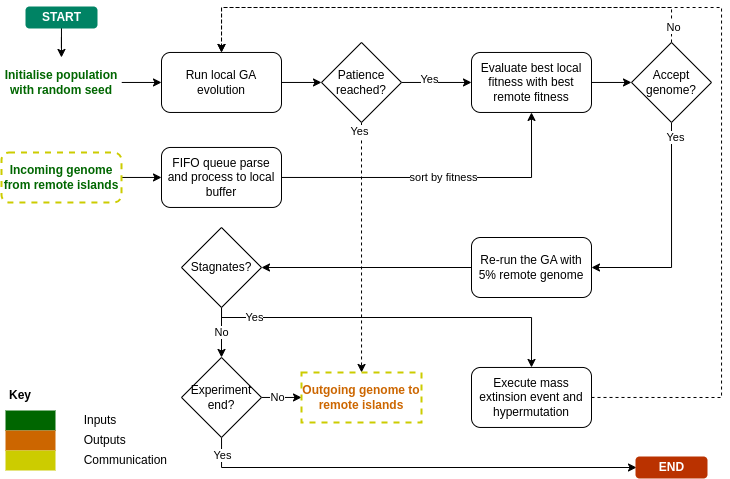
\includegraphics[width=0.65\textwidth]{ga.png}
    \caption{Island Model Flowchart}
    \label{fig:ga}
\end{figure*}

Our implementation employs an elitist migration strategy, this happens when the local GA reaches a patience threshold and the agent pushes its "best" (lowest fitness score) genome to other swarm members via ESP-NOW. The incoming remote genes from another peer are integrated into the local population by replacing the worst performing $5\%$ individuals, this value was chosen to preserve genomic high locally.\\ 

To avoid stagnation over a local-minimum, a mass extinction event together with a hyper-mutation mechanism tracks consecutive non-improving generations. Once a set of conditions is reached (Table X), the mutation probability is temporarily increased to escape local optima and lowest performing half of the population is re-initialised. This is done to promote exploration across the swarm and prevent premature convergence. 

\subsection{Real Time Operating System}

Each swarm member boots into a FreeRTOS runtime by calling \texttt{app\_main()}, which performs the initialisation of the following components: non-volatile storage, I2C peripherals, RTC, SD card, and ESP-NOW.

Figure \ref{fig:rtos} illustrates the sequence of these and their relation to the tasks that are spawned during run time. These tasks include:

\begin{itemize}
  \item \texttt{i2c\_task}: Handles communication with the $I^2C$ peripherals, including the AXP192 power supply, the IR board, the display and the Pololu 3pi+.
  \item \texttt{gui\_task}: Manages the UI on the M5Stack display, used for real-time feedback and debugging.
  \item \texttt{pololu\_heartbeat\_task}: Handles the $I^2C$ signal from the Pololu 3pi+, ensuring that the robot is operational and responsive.
  \item \texttt{ota\_task}: Manages OTA updates if a new version is available in S3 (Section \ref{sec:ota}).
  \item \texttt{espnow\_task}: Manages ESP-NOW communication between swarm members, handles message sending and receiving.
  \item \texttt{ga\_task}: Runs the local GA and coordinates with other tasks to log and transmit data.
  \item \texttt{write\_task}: Handles SD card operations, including data logging, managing file storage and uploading experimental results.
\end{itemize}

\begin{figure}[H]
    \centering
    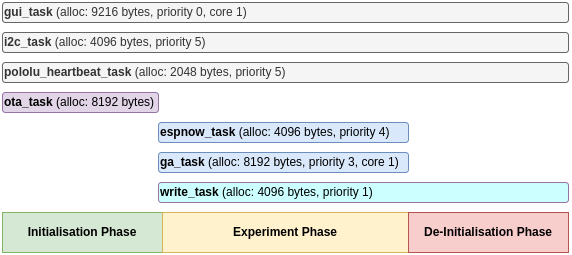
\includegraphics[width=0.48\textwidth]{rtos.png}
    \caption{Task schedule with memory allocation and priority.}
    \label{fig:rtos}
\end{figure}

Inter-task coordination is managed by event groups and queues. The event groups are used to signal task completion and synchronise downstream operations, whereas queues are used to pass data between tasks that are operating in parallel. This enables multitasking and real-time processing of the measurements.\\ 

Note that the local population undergoes evolution until the experiment phase is terminated. The experiment phase is terminated when one of the following criteria is met:

\begin{enumerate}
  \item \textbf{Global solution}: Any robot attains the exact global minimum of the Rastrigin function (fitness\,=\,0).
  \item \textbf{Time limit}: A maximum duration of 60 seconds elapses without global convergence.
\end{enumerate}

Upon reaching the de-initialisation phase, the \texttt{espnow\_task} drains pending message queues, final fitness and communication metrics are uploaded to an Amazon S3 bucket via HTTPS via the \texttt{write\_task}. Finally, the system peripherals are de-initialised to ensure a clean shutdown.

\subsection{Communication Layer}\label{sec:comm-layer}

We implemented ESP-NOW by pre-registering the MAC addresses for all peers in each agent, enabling direct unicast communication between swarm robots. Our design uses push only event-driven peer-to-peer messaging, where each device transmits data to peers without waiting for requests. Using this scheme avoids the complexity of pull-based communication protocols. Recall that once a local elite genome is found, the best solution is sent to all peers, if there are incoming messages these are queued for later processing, allowing task operations to continue uninterrupted. In this section we describe the specific communication independent variables that were manipulated during experiments.\\

\subsubsection{Topology Inference}\label{sec:topology-inference}

%We combine these insights by randomizing per-to-peer send times to desynchronize traffic, with one key difference: the maximum delay %time is capped by the measured ESPNOW latency between individual peers. It is worth noting that the RSSI is measured between peers and therefore it can be used as an indicative measure of the distance between agents though we also expect that the RSSI will be affected by the environment and obstacles in between the agents.

We investigate the impact of different communication schemes on the emergent swarm topology by introducing two distinct message transmission strategies: \textbf{STOCHASTIC} and \textbf{COMM\_AWARE}. Implemented in the communication layer, these were designed to influence the order and priority with which each agent sends data to its peers. The aim is to understand how these strategies affect the connectivity and robustness of the swarm network.\\

These are implemented as follows:

\begin{itemize}
    \item \textbf{STOCHASTIC}: Each agent calls a random seed to apply a Fisher-Yates shuffle over the list of peer MAC addresses to sort them before sending its message. This ensures that the order of communication is random for each transmission cycle, preventing biases.
    \item \textbf{COMM\_AWARE}: Each agent ranks its peers based on the most recent measurements of communication quality, specifically the last known latency and Received Signal Strength Indicator (RSSI). Peers with unknown metrics (during initialisation) are prioritized first to ensure all peer links are measured. Then, peers are scored by normalizing both latency and RSSI, and those only in the worst half (highest latency, lowest RSSI) are prioritized for message transmission.
\end{itemize}

The following pseudocode outlines the logic for each scheme:

%\paragraph{STOCHASTIC}
\begin{algorithm}[H]
\caption{Randomized Peer Selection}
\begin{algorithmic}[1]
\State \textbf{Input:} List of peer MAC addresses
\State Fisher-Yates shuffle using a random seed
\For{each peer in shuffled list}
    \If{peer is not self}
        \State Send message to peer
    \EndIf
\EndFor
\end{algorithmic}
\end{algorithm}

%\paragraph{COMM\_AWARE}
\begin{algorithm}[H]
\caption{Communication-Aware Peer Ranking}
\begin{algorithmic}[1]
\State \textbf{Input:} List of peer MAC addresses, last known RSSI and latency for each peer
\For{each peer}
    \If{RSSI or latency is null}
        \State Assign highest priority
    \Else
        \State Normalize RSSI and latency across all peers
        \State Compute score: $score = norm\_latency + norm\_rssi$
    \EndIf
\EndFor
\State Sort peers: null metrics first, then by descending score (worst first), only \textbf{50\% scope of network}
\For{each peer in sorted list}
    \If{peer is not self}
        \State Send message to peer
    \EndIf
\EndFor
\end{algorithmic}
\end{algorithm}

Note that these schemes are specifically designed for \textbf{unicast} communication, where messages are sent directly to individual peers and round-trip latency can be measured via acknowledgements (ACKS). Having said that, we can think of the \textbf{STOCHASTIC} algorithm as a pseuso-broadcast communication scheme as the message is sent to all peers with negligible delays between transmissions.\\ 

\subsubsection{Limited-Rate Communication}\label{sec:limited-rate}

Inspired by the “less-is-more” effects reported by \cite{aust_hidden_2022} using infrared links, we implemented a token-bucket limiter to the ESP-NOW layer and treat this quota as an independent variable. Each agent is given a small budget of 1 message in a sliding window of length 8 seconds.  When the bucket is empty the agent must keep silent until the window refreshes, regardless of how often its GA stagnates or improves.  This caps the total interaction rate per robot rather than solely spacing individual transmissions.

\begin{algorithm}[H]
\caption{Token-Bucket Throttled Send}
\label{alg:token_bucket}
\begin{algorithmic}[1]
\Require 
  $B$: message budget per window, \quad
  $W$: window length (ms), \quad
  $t_{\mathrm{last}}$: window start time, \quad
  $\mathit{tokens}$: remaining sends
\Procedure{MaybeSend}{$\mathit{payload}$}
  \State $now \gets$ \Call{CurrentTimeMs}{}
  \If{$now - t_{\mathrm{last}} \ge W$} \Comment{Window refresh}
    \State $\mathit{tokens} \gets B$
    \State $t_{\mathrm{last}} \gets now$
  \EndIf
  \If{$\mathit{tokens} = 0$}
    \State \Return \Comment{Bucket empty → no send}
  \EndIf
  \If{\Call{ImprovedFitness}{}}
    \State $\mathit{tokens} \gets \mathit{tokens} - 1$
    \State \Call{ESP\_NOW\_Send}{$\mathit{payload}$}
  \EndIf
\EndProcedure
\end{algorithmic}
\end{algorithm}

\subsubsection{Transmission Frequency}\label{sec:transmission-frequency}

To further explore the communication behaviour of the swarm under flooding conditions, we modulate the transmission frequency. In this communication mode, each message transmission is delayed by a random interval, otherwise no delay is explicitly applied. This random delay, drawn from a range determined by the maximum observed latency among peers, is described by Algorithm \ref{alg:transmission_freq}.\\

\begin{algorithm}[H]
\caption{Stochastic Transmission Frequency}
\label{alg:transmission_freq}
\begin{algorithmic}[1]
\State \textbf{Input:} List of peer MAC addresses, maximum latency observed ($max\_rand$)
\For{each peer in the target list}
    \If{peer is not self}
        \State Compute a random delay: $delay \gets rand(0, max\_rand)$
        \State Wait for $delay$ milliseconds
        \State Send message to peer
    \EndIf
\EndFor
\end{algorithmic}
\end{algorithm}

In the firmware, this is implemented by checking if \texttt{DEFAULT\_MIGRATION\_FREQUENCY} is set to \texttt{FREQUENCY\_RANDOM} and, if so, randomly delaying each call to \texttt{esp\_now\_send} by a value within the range of $[0, max\_rand]$, where $max\_rand$ is derived from the maximum measured latency among peers. The intention of this approach is to control the flooding of messages in a stochastic manner that can help reduce unintended collisions in the swarm network.

\subsection{Data Logging}\label{sec:data-logging}

Reliable and precise data logging is a pre-requisite for evaluating the communication performance and evolution dynamics of the swarm. To achieve this, our firmware implements several mechanisms to capture and record key metrics such as latency, message exchanges, internal state changes, and experiment metadata. These measurements are logged using well-defined data structures and are incrementally written to an SD card.\\

\subsubsection{Messaging Structure}

Table \ref{tab:out_message} summarizes the \texttt{out\_message\_t} structure used for transmitting messages between swarm peers via ESP-NOW. Note that any floating point values in the message content are rounded to $3 d.p.$ to ensure compact representation. The total size of the struct is kept within the raw payload limits (250 bytes) imposed by ESP-NOW to guarantee reliable transmission.

\begin{table}[h]
  \centering
  \caption{Message Structure (\texttt{out\_message\_t}) for ESP-NOW Data Transfer}
  \label{tab:out_message}
  \begin{tabular}{l l p{4cm}}
    \toprule
    \textbf{Field} & \textbf{Type} & \textbf{Description} \\
    \midrule
    \texttt{log\_id} & uint32\_t & Unique internal identifier of the event.\\
    \texttt{robot\_id[5]} & char & MAC identifier for the sender robot plus a null terminator.\\
    \texttt{created\_datetime} & time\_t & Timestamp based on the internal RTC.\\
    \texttt{message[128]} & char & Content of the message including the fitness score and genome delimited by "$|$".\\
    \bottomrule
  \end{tabular}
\end{table}

\subsubsection{Data Processing}

The data logging pipeline is designed to ensure that all key experimental metrics are captured and preserved locally by each agent. Log entries are posted to two FreeRTOS queues: \texttt{LogQueue} for internal logging events and \texttt{LogBodyQueue} for detailed message logs. A \texttt{QueueSet} allows the dedicated \texttt{write\_task} to efficiently monitor and process both queues in real time.\\

The core logging framework relies on three primary data structures:
\begin{itemize}
    \item \texttt{experiment\_metadata\_t}: Stores overall experiment parameters, including experiment and robot IDs, random seed, GA parameters, migration settings, and application version.
    \item \texttt{event\_log\_t}: Used for logging system events such as latency measurements, RSSI, CPU usage, and state changes.
    \item \texttt{event\_log\_message\_t}: Holds the parsed version of the \texttt{out\_message\_t} structure and links it to the internal event ID.
\end{itemize}

When an entry is retrieved from either queue, it is serialized into a JSON-formatted string (via \texttt{serialize\_log\_to\_json()}) to ensure structured and consistent downstream analysis. The serialized data is then written incrementally to SD card files, with each file capped at 1MB to prevent memory overflow and ensure robust storage. Figure~\ref{fig:data-store} illustrates the internal data logging pipeline, from event generation to SD card storage.

\begin{figure}[H]
    \centering
    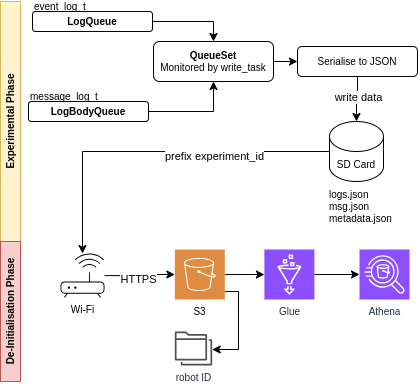
\includegraphics[width=0.45\textwidth]{data_store.png}
    \caption{Internal data logging pipeline}
    \label{fig:data-store}
\end{figure}

After the experimental phase concludes, the system enters a data upload mode. In this mode, the files stored on each agent's SD cards are uploaded to an AWS S3 bucket via HTTPS. This was done by design as we did not want to stream the data from the peers whilst they were running the experiment, as this could have introduced additional collisions potentially impacting the measurements.\\

As depicted by Figure \ref{fig:data-store}, the S3 bucket is structured to store each agent's data in a separate folder, named by the robot's ID. Each file is named with a timestamp and the experiment ID, ensuring that all data is uniquely identifiable and traceable. The data is then processed using AWS Glue to prepare it for analysis using Amazon Athena. This process allowed us to automate the storage and evaluation of data logs from over $500$ experiment runs.

\subsection{Communication Performance Metrics}

To evaluate the quality of network communication in the swarm, the following metrics were computed, (i) $L$ \emph{latency (ms)}, the time taken for a message to be sent and acknowledged by a peer, (ii) $J$ \emph{jitter (ms)}, the variation in latency between messages, (iii) $P$ \emph{packet loss (\%)}, the percentage of messages that were sent but not acknowledged, and (iv) $T$ \emph{throughput (kbps)}, the rate at which data is successfully sent and received by each agent.

To assess overall network performance, a Quality of Service (QoS) score was computed for each run using a weighted sum of normalized network metrics. The equation is defined as:

\begin{equation}
\mathrm{QoS} = w_0 \cdot (1 - \hat{L}) + w_1 \cdot (1 - \hat{J}) + w_2 \cdot (1 - \hat{P}) + w_3 \cdot \hat{T}
\end{equation}

Here, each metric is normalized to the range [0,1] and the weights $w_i$ are defined in Table \ref{tab:qos}. A higher QoS value indicates better overall network communication performance.

\begin{table}[H]
\centering
\caption{QoS utility function weights for different swarm robotics applications}
\label{tab:qos}
  \begin{tabular}{@{} lcccc p{3.5cm} @{}}
  \toprule
  \textbf{QoS} & \textbf{$w_0$} & \textbf{$w_1$} & \textbf{$w_2$} & \textbf{$w_3$} & \textbf{Application} \\
  \midrule
  $QoS_c$      & 0.5 & 0.25   & 0.15   & 0.1     & Swarm consensus and voting     \\
  $QoS_s$      & 0.3 & 0.15   & 0.45   & 0.1     & Swarm sparse deployments       \\
  \bottomrule
  \end{tabular}
\end{table}

\section{Preliminary Analysis}

Using a single robot, a preliminary analysis was conducted to identify suitable parameters for solving the Rastrigin function under varying population sizes (10, 20) and gene dimensions (2, 3, 4, 5). Over 100 experimental runs were performed, each terminating if fitness failed to improve beyond a 0.001 threshold over 20 consecutive epochs. As shown in Figure \ref{fig:ga_prelim_analysis}, larger populations yielded lower median fitness scores.

\begin{figure}[h]
    \centering
    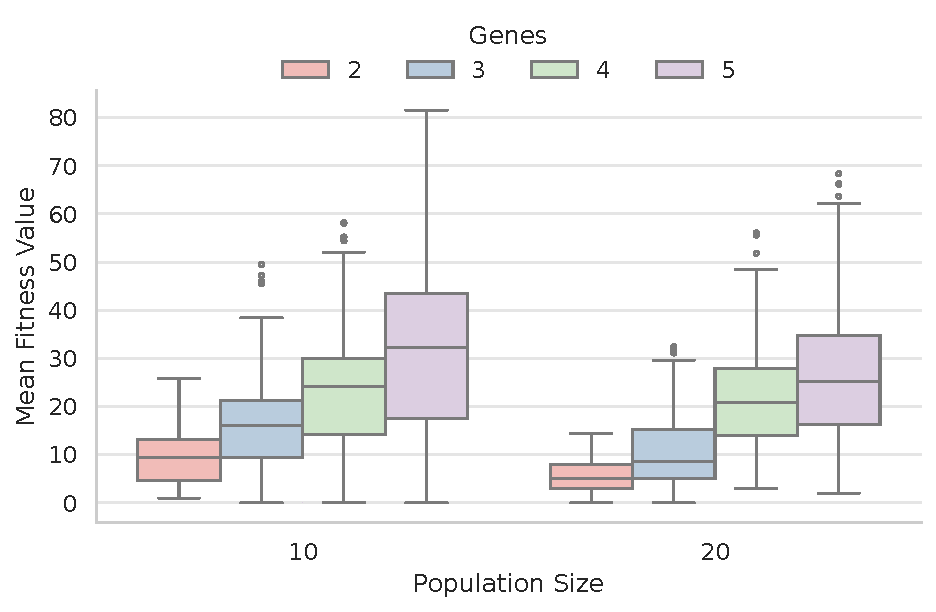
\includegraphics[width=0.47\textwidth]{ga_prelim_analysis_v2.pdf}
    \caption{Fitness distribution by population size and gene dimensionality}
    \label{fig:ga_prelim_analysis}
\end{figure}

The time taken to converge ranged between 0 to 3 seconds, reflecting the early stopping triggered by the patience setting. The data gathered from these early experiments suggested that using five genes was not sufficiently challenging for a single agent as convergence was achieved too quickly. Due to this we decide to expand the Rastrigin search dimensionality to 10 genes and extend the local population and threshold epochs to 60. Hypermutation parameters are also set at this stage and implemented the most practical experiment run time, firmware improvements are summarised in Table \ref{tab:firmware_versions}.

\begin{table}[H]
\centering
\caption{Firmware updates and change log}
\begin{tabular}{@{} l p{7.5cm} @{}} 
\toprule
\textbf{Version} & \textbf{Notes} \\
\midrule
v0.3 & Single agent experiments, GA parameter tuning. \\
v0.4 & Improved late message queue handling. Use 10 Genes.\\
v0.5 & Reduced experiment time from 120 seconds to 60 seconds. \\
v0.6 & Increased queue size to 40 (previously 25), to ensure no messages are lost.\\
\bottomrule
\end{tabular}
\label{tab:firmware_versions}
\end{table}

With two agents, we built a baseline shown in Table \ref{tab:exp_config}. The dual agents did not reach the global minimum in these trials, but consistently converged to a local minimum within the first 20 seconds of the experimental phase.

\section{Results}

As shown in Figure \ref{fig:topology}(a), the latency and jitter of the swarm network differ significantly between topology inference schemes. Across experiments the \emph{COMM AWARE} topology strategy generally achieves lower latency and more stable delivery compared to the \emph{STOCHASTIC} mode. Figures \ref{fig:topology}(b) and \ref{fig:topology}(c) show that throughput is highest in unconstrained conditions, and drops with the introduction of message budgets. \emph{STOCHASTIC} communication yields higher raw throughput but also has a wider range of variability.

\begin{figure*}[h]
    \centering
    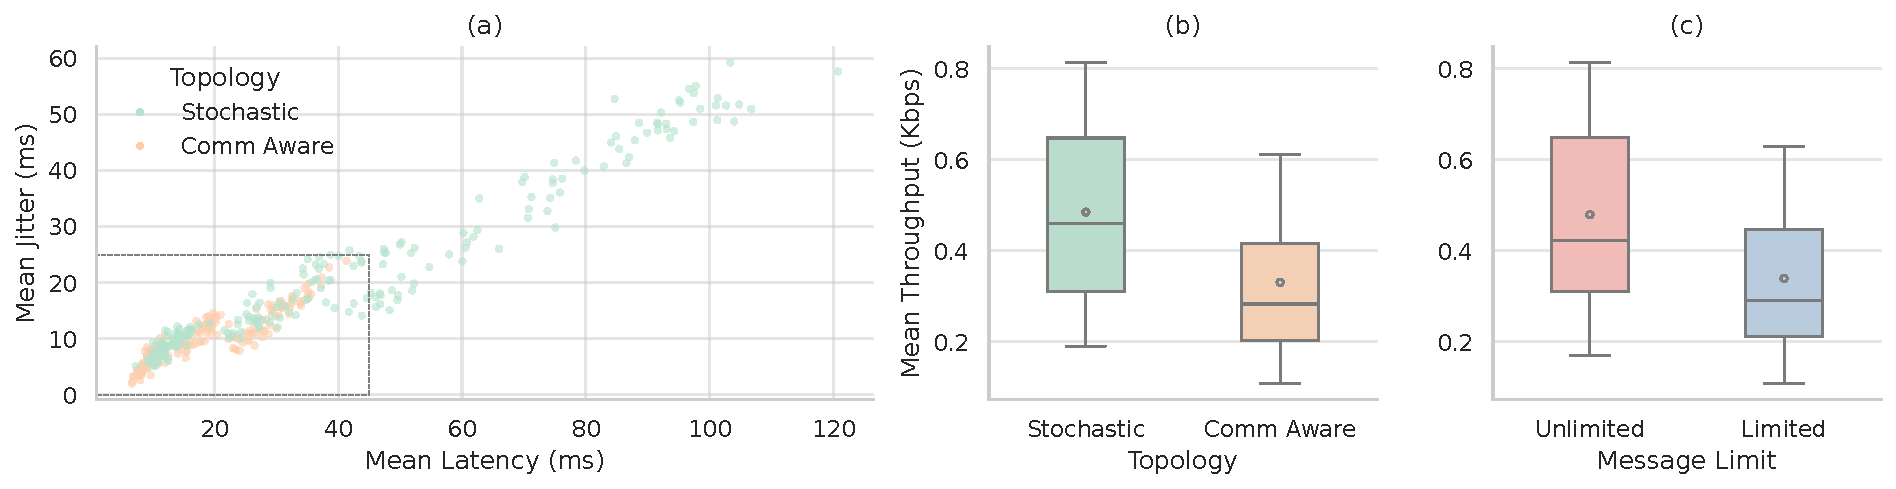
\includegraphics[width=1\textwidth]{topology_impact.pdf}
    \caption{(a) Latency and Jitter relationship under varying topology schemes, (b)(c) throughput distribution under topology and message limit variables}
    \label{fig:topology}
\end{figure*}

Figure \ref{fig:performance}(a) shows that larger swarms converge to lower mean fitness scores, indicating improved global convergence as agent density increases. Figure \ref{fig:performance}(b) presents the adaptation rate over time. Swarms using the \emph{STOCHASTIC} communication scheme tend to converge more rapidly, with approximately $80\%$ of the agents reaching the best-known solution roughly 20 seconds earlier than those using the \emph{COMM AWARE} strategy. Here, adaptation rate is defined as the proportion of agents that share the current lowest fitness score, averaged over 2-second windows.

\begin{figure*}[h]
    \centering
    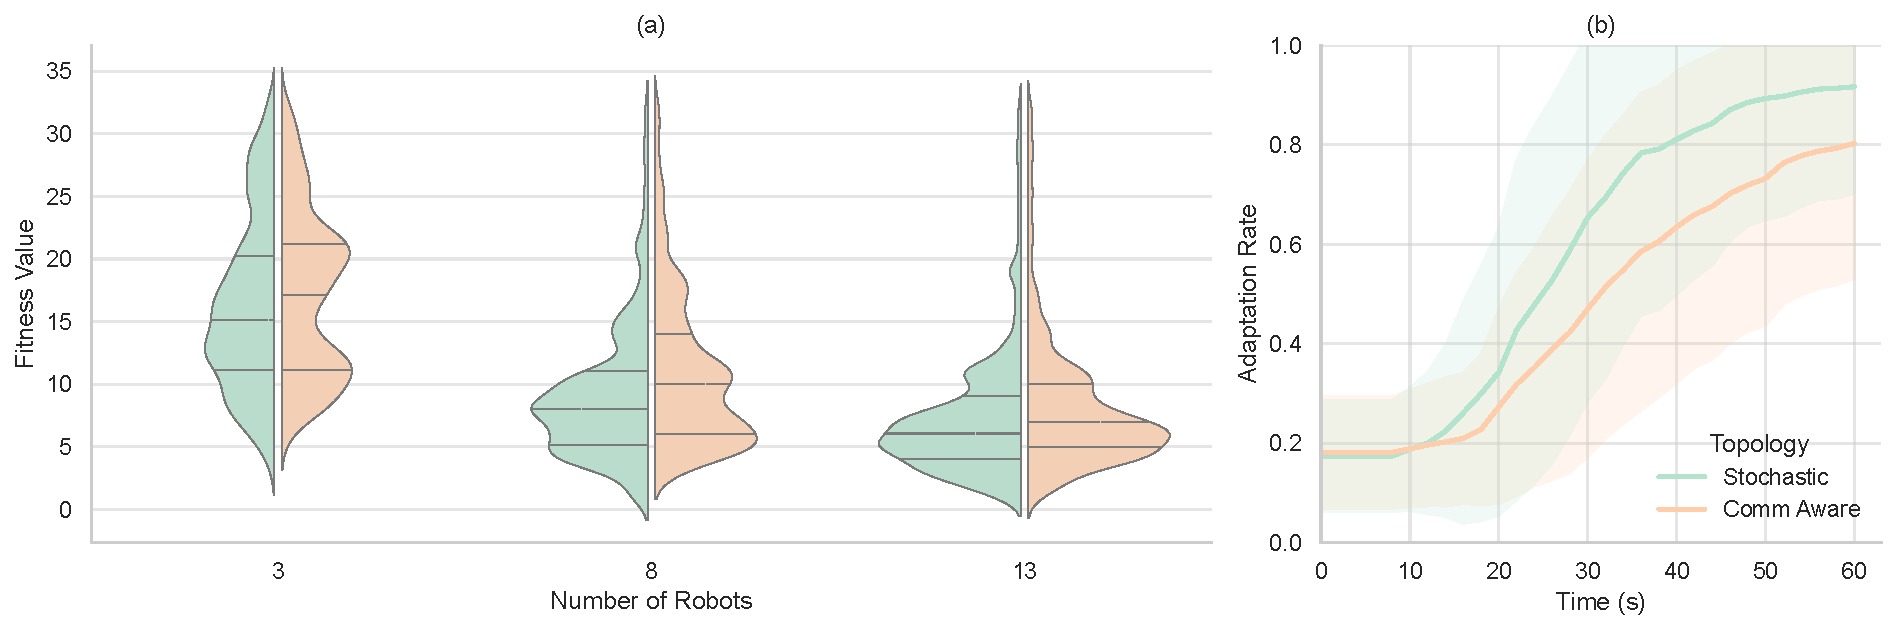
\includegraphics[width=1\textwidth]{performance_impact.pdf}
    \caption{(a) Mean device fitness values across different swarm sizes, (b) mean cumulative percentage of agents converging to the lowest fitness value across $2s$ windows}
    \label{fig:performance}
\end{figure*}

Figure \ref{fig:error-rates}(a) shows the mean packet error rate across different swarm densities. The error rates remain low overall but increase with the swarm size, and it is particularly impacted by the \emph{STOCHASTIC} scheme (Figure \ref{fig:error-rates}(b)).

\begin{figure}[H]
    \centering
    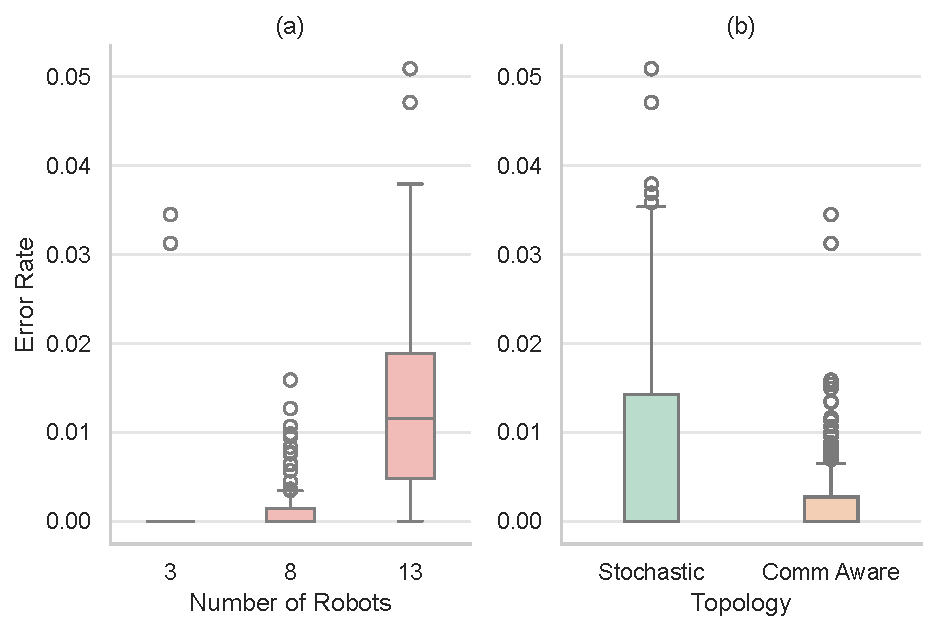
\includegraphics[width=0.47\textwidth]{reliability_impact.pdf}
    \caption{(a) Mean error rates by device across varying swarm sizes, (b) mean error rate for different topology inference schemes}
    \label{fig:error-rates}
\end{figure}

With regards to locomotion Figure \ref{fig:rssi}(a) shows that Brownian motion results in slightly improved RSSI values, indicating more stable connections compared to static swarms. Whereas \ref{fig:rssi}(b) suggests no statistical difference between RSSI values across topology inference schemes.

\begin{figure}[H]
    \centering
    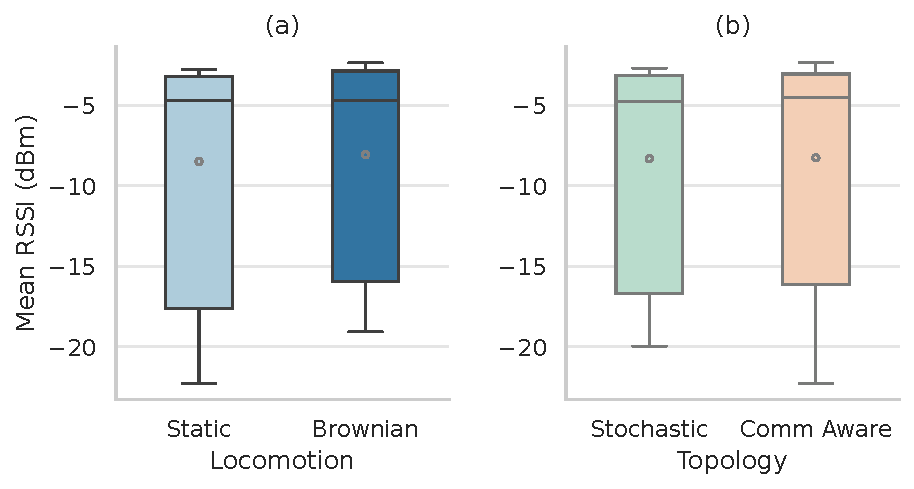
\includegraphics[width=0.47\textwidth]{speed_impact.pdf}
    \caption{(a) Mean RSSI values across different locomotion modes, (b) mean RSSI values accross different topology inference schemes}
    \label{fig:rssi}
\end{figure}

Considering the impact of transmission frequency for experiments under the STOCHASTIC scheme, Figure \ref{fig:frequency}(a) shows that modulated transmission policies also restrict the network to lower latency and jitter though not to the same degree. Figure \ref{fig:frequency}(b) illustrates how latency varies over time under different transmission settings, with modulated policies achieving lower more stable latencies. Figure \ref{fig:frequency}(c) shows that throughput is generally similar between policies, a contrast compared to the topology inference schemes. Similar to performance under varying topology inference conditions, the performance for alternating transmission policies remains impacted mainly by the increase in swarm density Figure \ref{fig:f-performance}(a). Moreover, the adaptation rate between transmission policies remains similar Figure \ref{fig:f-performance}.\\

\begin{figure*}[h]
    \centering
    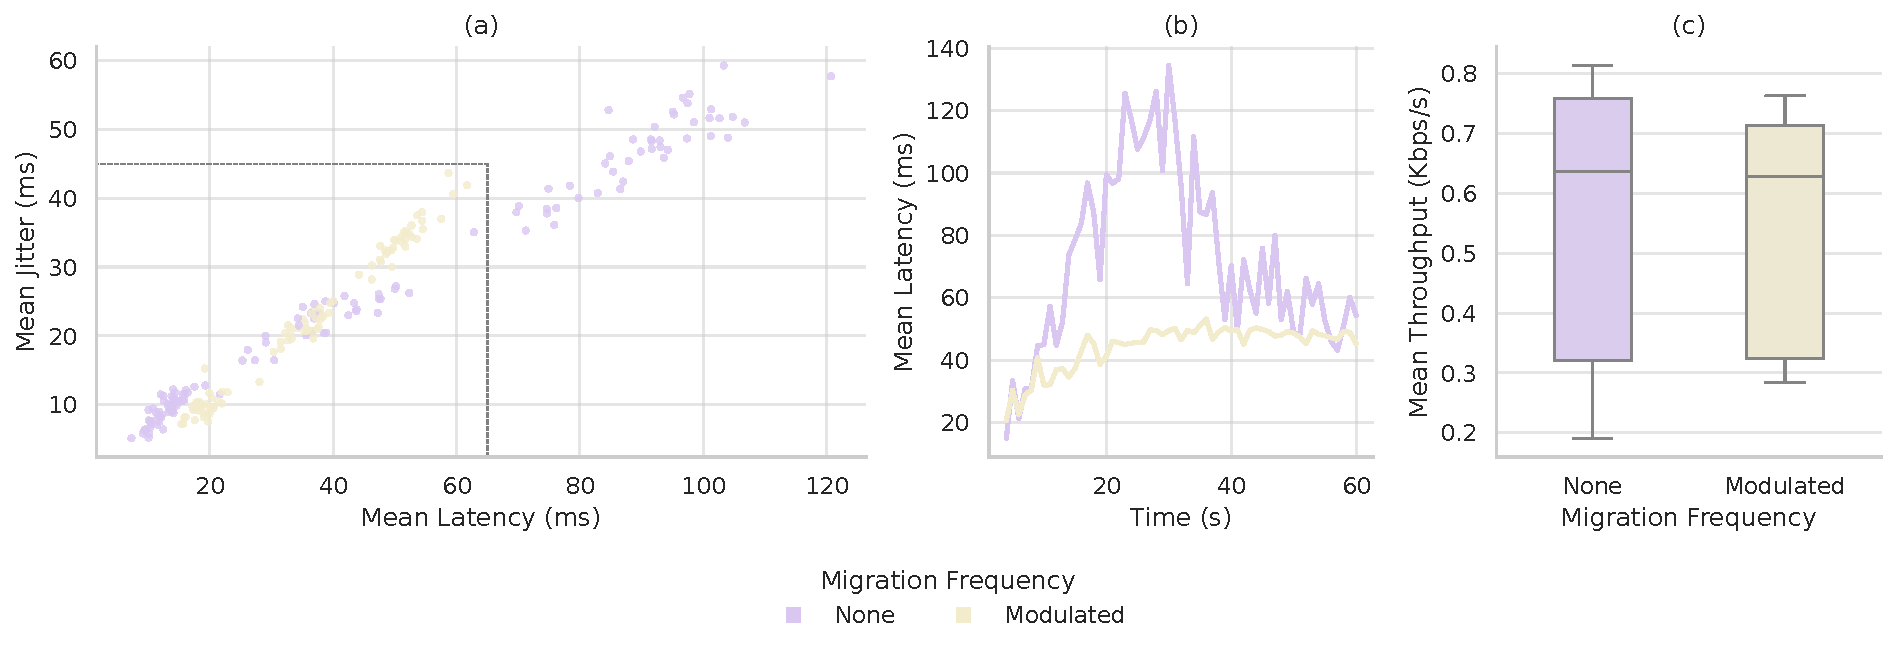
\includegraphics[width=1\textwidth]{frequency_impact.pdf}
    \caption{(a) Latency and Jitter relationship under varying transmission policies, (b) latency across time by transmission setting, (c) throughput distribution by transmission setting}
    \label{fig:frequency}
\end{figure*}

\begin{figure*}[h]
    \centering
    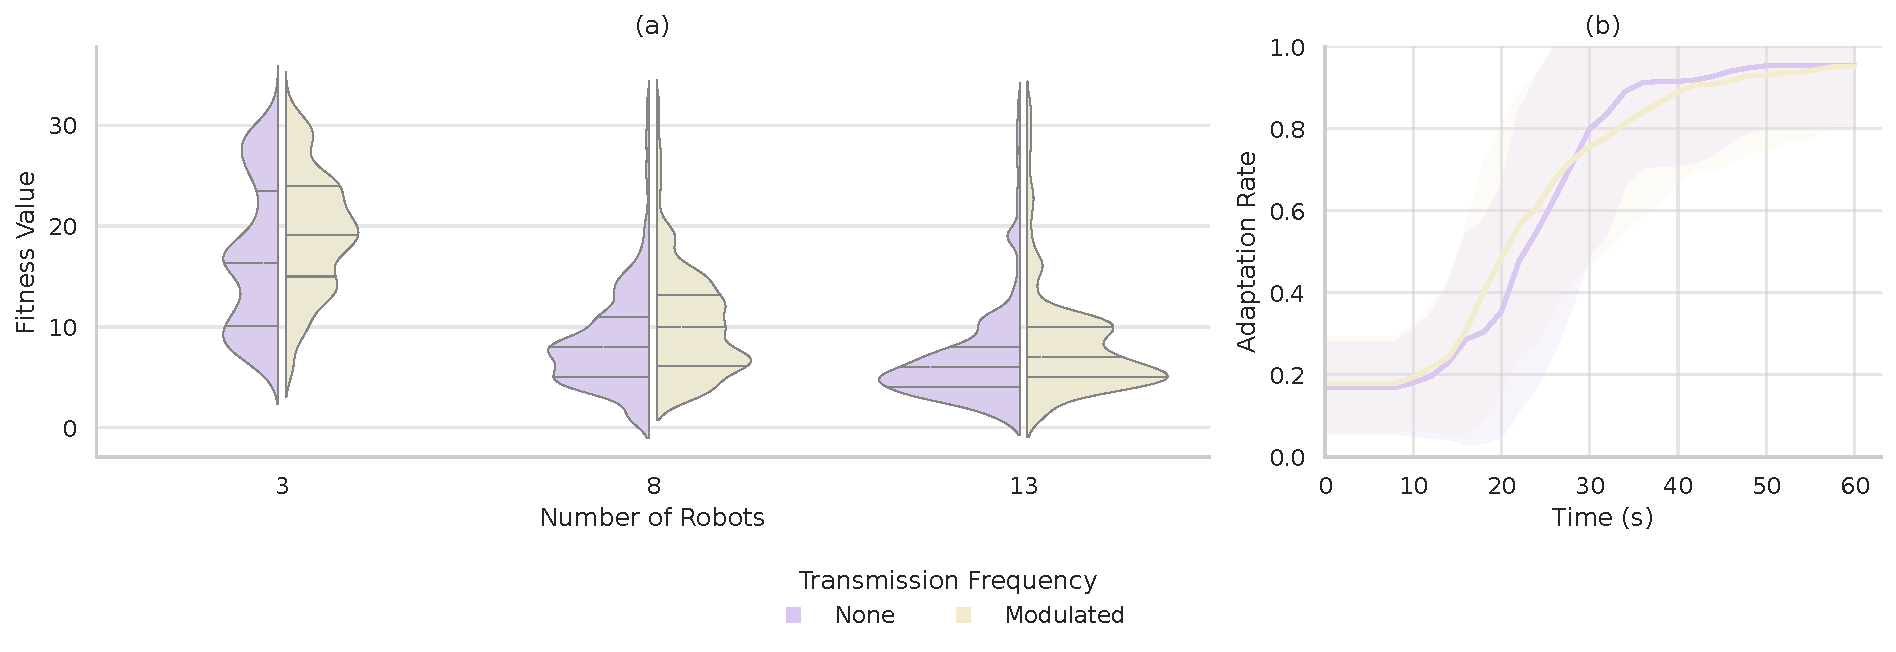
\includegraphics[width=1\textwidth]{f_performance_impact.pdf}
    \caption{(a) Mean device fitness values across different swarm sizes, (b) mean cumulative percentage of agents converging to the lowest fitness value across $2s$ windows}
    \label{fig:f-performance}
\end{figure*}

An evaluation of the characteristics of the QoS metrics for the 13-agent swarm is shown in Figure \ref{fig:qos}. Key observations include, (i) COMM AWARE topology inference achieves high QoS metrics, (ii) modulated transmission also scores high in QoS but tends to score higher in $QoS_s$, (iii) message limits do not have a clear effect on QoS, both kernel densities overlap each other.

\begin{figure*}[h]
    \centering
    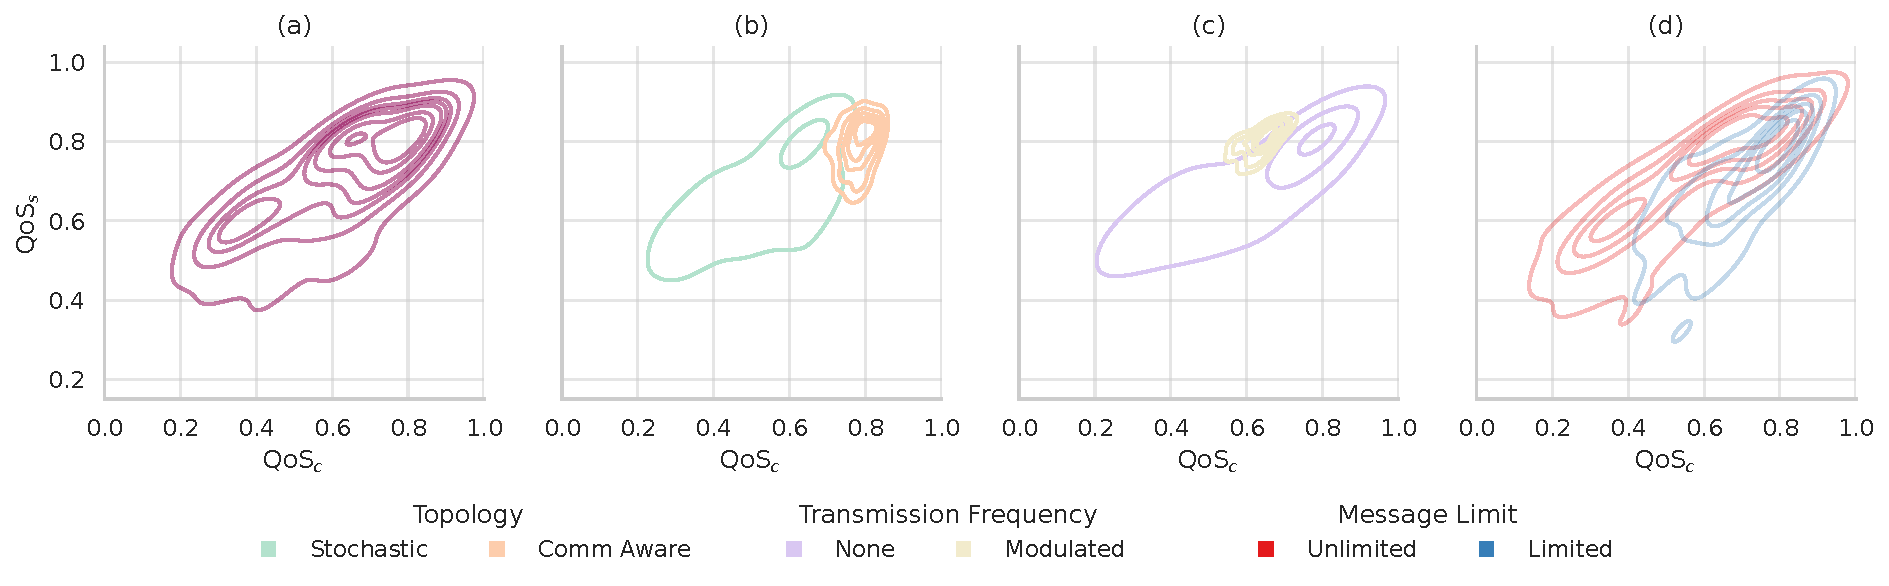
\includegraphics[width=1\textwidth]{qos_impact.pdf}
    \caption{Kernel-density contours showing the joint distribution of two QoS metrics (x: $QoS_c$, y: $QoS_s$) for a 13-agent swarm. (a) pooled across all experimental factors, (b) split by communication topology, (c) split by transmission frequency policy, (d) split by message limit setting}
    \label{fig:qos}
\end{figure*}

\renewcommand{\arraystretch}{0.9}  
\begin{table*}[ht]
\scriptsize
\centering
\caption{Experimental configurations}
\label{tab:exp_config}
\begin{tabular}{c|c|c|c|c|c|c|c|c|c|c}
\toprule
\textbf{Robots} & \textbf{Topology} & \textbf{Locomotion} & \textbf{Message Limit} & \textbf{Transmission} & \textbf{Latency (ms)} & \textbf{Jitter (ms)} & \textbf{Error Rate (\%)} & \textbf{Throughput} & \textbf{QoS\_c} & \textbf{QoS\_s} \\
\midrule
2 (Baseline) & Stochastic & Static & Unlimited & None & -- & -- & -- & -- & -- & -- \\
\midrule
\multirow{10}{*}{3}
  & \multirow{5}{*}{Stochastic}
    & \multirow{2}{*}{Static}
                 & Unlimited & None      & -- & -- & -- & -- & -- & -- \\
  &   &          & Unlimited & Modulated & -- & -- & -- & -- & -- & -- \\
  &   &          & Limited   & None      & -- & -- & -- & -- & -- & -- \\
  \cmidrule{3-11}
  &   & \multirow{2}{*}{Brownian}
                 & Unlimited & None      & -- & -- & -- & -- & -- & -- \\
  &   &          & Unlimited & Modulated & -- & -- & -- & -- & -- & -- \\
  &   &          & Limited   & None      & -- & -- & -- & -- & -- & -- \\
  \cmidrule{2-11}
  & \multirow{5}{*}{Comm Aware}
    & \multirow{2}{*}{Static}
                 & Unlimited & None      & -- & -- & -- & -- & -- & -- \\
  &   &          & Limited   & None      & -- & -- & -- & -- & -- & -- \\
  \cmidrule{3-11}
  &   & \multirow{2}{*}{Brownian}
                 & Unlimited & None      & -- & -- & -- & -- & -- & -- \\
  &   &          & Limited   & None      & -- & -- & -- & -- & -- & -- \\
\midrule
\multirow{10}{*}{8}
  & \multirow{5}{*}{Stochastic}
    & \multirow{2}{*}{Static}
                 & Unlimited & None      & -- & -- & -- & -- & -- & -- \\
  &   &          & Unlimited & Modulated & -- & -- & -- & -- & -- & -- \\
  &   &          & Limited   & None      & -- & -- & -- & -- & -- & -- \\
  \cmidrule{3-11}
  &   & \multirow{2}{*}{Brownian}
                 & Unlimited & None      & -- & -- & -- & -- & -- & -- \\
  &   &          & Unlimited & Modulated & -- & -- & -- & -- & -- & -- \\
  &   &          & Limited   & None      & -- & -- & -- & -- & -- & -- \\
  \cmidrule{2-11}
  & \multirow{5}{*}{Comm Aware}
    & \multirow{2}{*}{Static}
                 & Unlimited & None      & -- & -- & -- & -- & -- & -- \\
  &   &          & Limited   & None      & -- & -- & -- & -- & -- & -- \\
  \cmidrule{3-11}
  &   & \multirow{2}{*}{Brownian}
                 & Unlimited & None      & -- & -- & -- & -- & -- & -- \\
  &   &          & Limited   & None      & -- & -- & -- & -- & -- & -- \\
\midrule
\multirow{10}{*}{13}
  & \multirow{5}{*}{Stochastic}
    & \multirow{2}{*}{Static}
                 & Unlimited & None      & -- & -- & -- & -- & -- & -- \\
  &   &          & Unlimited & Modulated & -- & -- & -- & -- & -- & -- \\
  &   &          & Limited   & None      & -- & -- & -- & -- & -- & -- \\
  \cmidrule{3-11}
  &   & \multirow{2}{*}{Brownian}
                 & Unlimited & None      & -- & -- & -- & -- & -- & -- \\
  &   &          & Unlimited & Modulated & -- & -- & -- & -- & -- & -- \\
  &   &          & Limited   & None      & -- & -- & -- & -- & -- & -- \\
  \cmidrule{2-11}
  & \multirow{5}{*}{Comm Aware}
    & \multirow{2}{*}{Static}
                 & Unlimited & None      & -- & -- & -- & -- & -- & -- \\
  &   &          & Limited   & None      & -- & -- & -- & -- & -- & -- \\
  \cmidrule{3-11}
  &   & \multirow{2}{*}{Brownian}
                 & Unlimited & None      & -- & -- & -- & -- & -- & -- \\
  &   &          & Limited   & None      & -- & -- & -- & -- & -- & -- \\
\bottomrule
\end{tabular}
\end{table*}


\section{Discussion}
Results for our hypotheses are as follows. \textbf{H1} is supported: \emph{COMM AWARE} achieves lower median latency ($\delta$ XX ms) and tighter jitter than \emph{STOCHASTIC}. \textbf{H2} is partially supported: message budgets slow diffusion and curb collisions yet do not prevent convergence, however the effect size is modest compared with topology choice. \textbf{H3} is supported: a delay capped by recent peer latency reduces contention, stabilises latency (jitter $YY\%$), and maintains throughput relative to pure flooding.\\

Across conditions, reductions in end-to-end latency are explained mainly by the number of links the swarm forms rather than by capping the number of transmissions, achieving below $50ms$ comparable to simulation conditions in \cite{hauert_evolved_2009}. Under \emph{STOCHASTIC} scheduling the pseudo-broadcasting behaviour of the swarm rapidly increases unique connections, which raises contention. In \emph{COMM AWARE}, reduced link formation avoids bursts of transmission, producing lower median latency and jitter at the cost of throughput. The time-snapshots of inferred topologies in Fig. \ref{fig:convergence} illustrate this mechanism directly, with \emph{STOCHASTIC} creating denser transient link sets than \emph{COMM AWARE} over comparable intervals. In this elitist island-model, slower mixing between islands can be useful. Limiting link formation in \emph{COMM AWARE} reduces premature convergence, allowing for a more diverse genome to persist and be explored longer. This aligns with the observation that overall fitness improves primarily with agent count (Fig. \ref{fig:performance}a), while the fastest adaptation rates arise under the \emph{STOCHASTIC} scheme where information diffuses quickly (Fig. \ref{fig:f-performance}b).\\

% Results from the effects of the topology inference suggest that the primary driver in the reduction of latency <50ms is driven by the number of links being formed rather than the number of messages being limited. This is because although we observe a similar reduction in throughput for variables, the effect size over latency and jitter is not as pronounced when messages only budgeted. The concept that number of links formed over time drives latency reduction is elicidated in Figure \ref{fig:convergence}, which show the pseduo-flooding effect of the \emph{STOCHASTIC} scheme, over a similar time periods it yields more agents connecting to one-another whereas on the \emph{COMM AWARE} regime the formation of local pockets of information is possible due to the number of link formation being capped. The effect of having slower adaption rates in an elitist island model such as this one supports the idea that avoiding premature convergence between agents is beneficial from an evolutionary perspective, as it allows for more diverse genome to be explored for longer time spans. Conversely, overall fitness values for Rastrigin are mainly influenced by an increasing number of agents, supporting the theory that under more genetic variation results in an improved search.\\

\begin{figure*}[h]
    \centering
    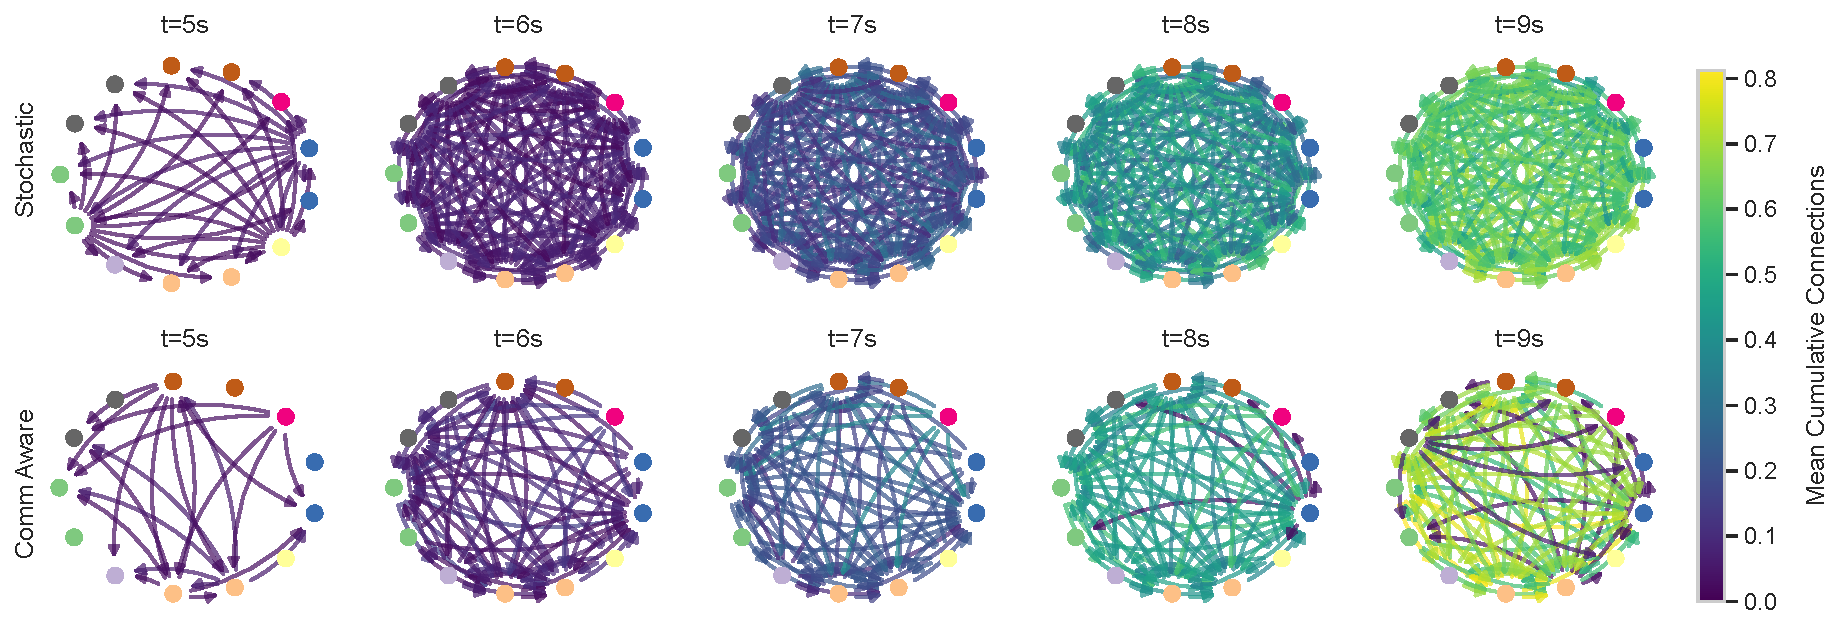
\includegraphics[width=1\textwidth]{convergence_impact.pdf}
    \caption{Temporal snapshots of inferred communication topologies for a 13-agent swarm. Rows: inference scheme, columns: time samples. Nodes are on a fixed circular layout, edges show inferred links and its colour indicates mean cumulative transmissions per node.}
    \label{fig:convergence}
\end{figure*}

\emph{COMM AWARE} attains consistently high $QoS$ values by suppressing jitter and keeping low latencies, while \emph{STOCHASTIC} achieves higher raw throughput but with wider variability and higher error rates as agent density grows. Kernel-density plots of $QoS_c$ against $QoS_cs$ in Fig. \ref{fig:qos} show \emph{COMM AWARE} achieving an overall improved service relative to the overall distribution, whereas frequency modulated \emph{STOCHASTIC} shifts mass toward $QoS_s$, reflecting higher throughputs with smoother latency over time.
Error rate increases with swarm size (Fig. \ref{fig:error-rates}), independent of locomotion, and becomes most pronounced under \emph{STOCHASTIC} at 13 robots—consistent with more concurrent transmissions and higher collision probability as unique links accumulate over time (Fig. \ref{fig:unique-connections}). This could explain why differences between policies are less pronounced at lower densities (3 to 8 robots) and widen at 13.\\

% The results suggest that using \emph{COMM AWARE} achieves high $QoS$ values as jitter and latency remain low whilst error rates are also abated, with the main trade off for this being a reduction in overall throughput of the network. Although not explicitly shown on the results one the key observations that we made is that the impact on $QoS$ scores is less varied on swarm densities below 13 agents, in which swarms of 3 and 8 scored high values irrespective of which variable was being isolated, this could potentially mean that at a particular swarm density collision rates become more prominent over the network as the number of connection increases (Figure \ref{fig:unique-connections}) . This is also supported by the fact that the error rates are higher in larger swarms (Figure \ref{fig:error-rates}).\\

\begin{figure}[H]
    \centering
    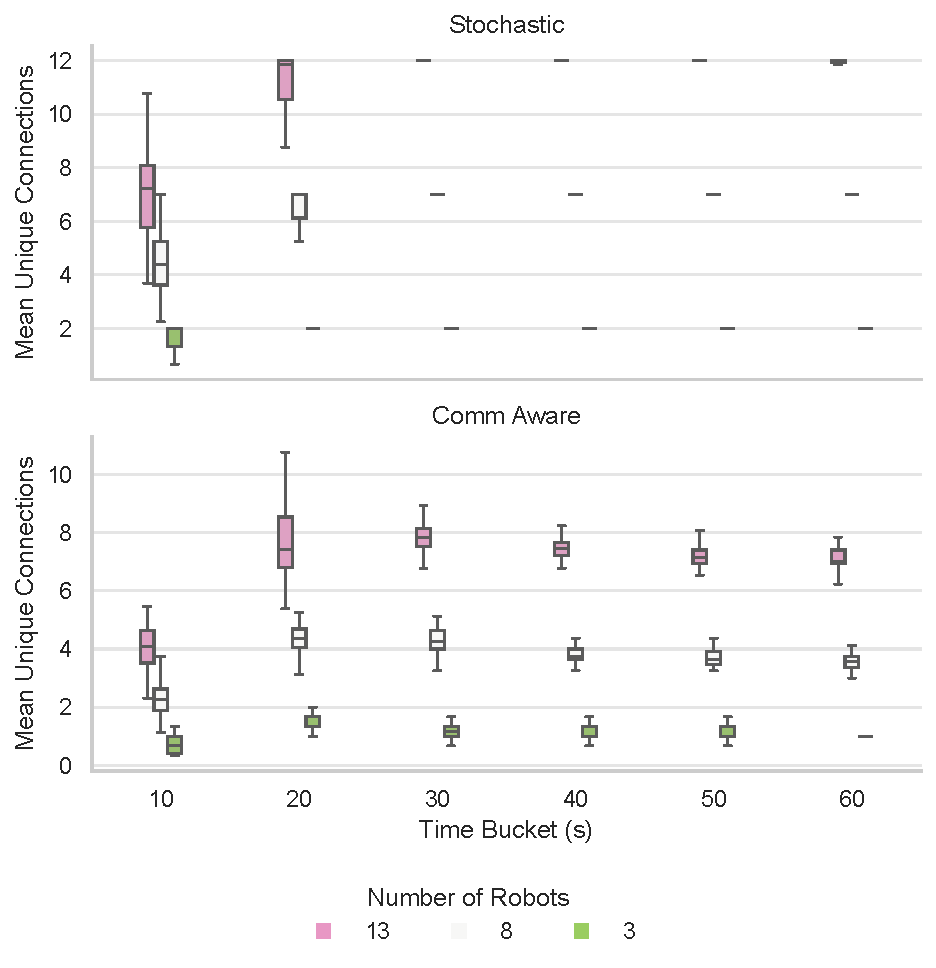
\includegraphics[width=0.46\textwidth]{unique_connections.pdf}
    \caption{Per-peer number of mean connections formed by time snapshot up to 30 seconds for both topology inference schemes}
    \label{fig:unique-connections}
\end{figure}

Results shown in Fig. \ref{fig:rssi}, indicate that RSSI does not meaningfully distinguish topology schemes in the arena used for the experiments, which means that the \emph{COMM AWARE} scheme is effectively ranking by latency. Brownian motion yields a slight RSSI improvement relative to static trials, plausibly by incidental repositioning into stronger links though verifying this would require sparser layouts or larger arenas.

% Regarding the effect of RSSI, results shows that during the experiments there was no significant difference between the topological inference schemes, this was expected as the maximun possible distance that the agents were sending messages across was around $~1m$, this means that the \emph{COMM AWARE} was mainly driven biased by latency instead of RSSI, further studies on sparse swarms would be needed to see if RSSI could be used in combination with latency to obtain similar results. Interestingly, we note a small effect in the improvement of RSSI values when Brownian locomotion is induced in the swarm, this is might be due to the fact that the agents are not stationary and therefore they are able to move around and find better communication links with their peers having said that further investigation is needed to fully understand this phenomenon.\\

Introducing frequency modulation under the \emph{STOCHASTIC} scheme smooths latency trajectories (Fig. \ref{fig:frequency}(b)) without sacrificing throughput, and preserves fast adaptation relative to \emph{COMM AWARE}. Validating the findings of \cite{tsianos_impact_2012}, the swarm can tolerate transmission delays and attain similar fitness relation compared to have no modulation. For tasks where rapid environment updates matter such as in \cite{perrin_decentralised_2012}, this policy provides a low complexity alternative to pure flooding, supported with a gentler latency profile.

% We observe that this type of communication policy shifts the $QoS$ scores towards $QoS_s$ that prioritises sensing tasks in a swarm that favor higher throughpus and lower error rates. In \cite{perrin_decentralised_2012}, we note that this type of communication might be beneficial in search and rescue operations where the goal is to quickly disseminate information about the environment and adapt to changing conditions.\\

Using the fixed ~145-byte genome structure (\texttt{OUT\_MESSAGE\_T}) in a single channel operation, we observe that GA performance is not capped by the aggregate throughput of the swarm. Having said that, we cannot ruleout the impact of a varying payload structure and single channel with respect to the GA without further experiments (e.g. partial genomes transfer, non-elitist migrants). Aditionally, more data would be needed to test whether the results gathered in this study remains the same as the messages grow closer to or beyond ESP-NOW 250-byte payload. We suspect that increasing the message size beyond the payload limits will introduce introduce challenges in asynchronous message processing as the local buffer would need to grow to prevent information loss and the subsequent compute requirements will increase as well.\\


% The evidence suggests that the throughput is not the primary limiting factor over the performance of the elitist island-model. The message OUT\_MESSAGE\_T that was exchanged by the swarm was kept constant with 10 genes and size of 145 bytes and transmitted over a single channel, yet we know from \cite{hauert_evolved_2009} that multiple channels can be used in swarms. We yet do not know what the impact of the data structure might have over the swarm's evolutionary performance and perhaps an extension of this work should investigate the impact of exchanging partial genomes and observe its effect on non-elitist GAs.  

Energy consumption matters. Broadcast-heavy policies increased CPU utilisation (Fig. \ref{fig:cpu-util}) and correlated with faster battery depletion during testing, whereas policies that constrain link formation (\emph{COMM AWARE}) reduced contention and processing load, extending runtime. For context, ESP-NOW transmit currents on ESP32 are typically an order of magnitude higher than BLE ($\approx100mA$ vs $\approx15mA$ during TX), so depending on the application, swarms may need to prioritise message budgets and partial link formation over peak performance. This trade-off is not abstract, in the author's current role at Unilode Aviation Solutions the operator of the largest globally distributed aviation IoT gateway network—battery longevity outranks other $QoS$ metrics because asset maintenance for sparsely distributed assets (agents) is measured in years rather than days.\\

\begin{figure}[H]
    \centering
    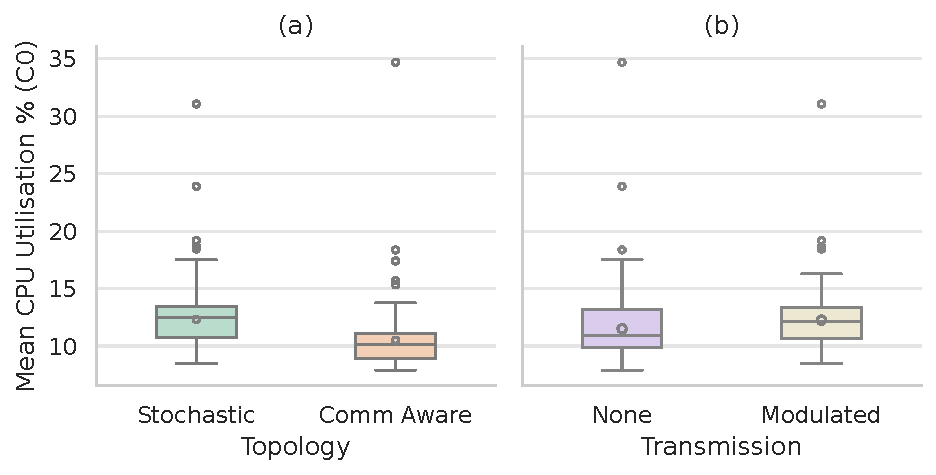
\includegraphics[width=0.46\textwidth]{cpu_util.pdf}
    \caption{Core 0 utilisation by communication policy, excluding message limited experiments}
    \label{fig:cpu_util}
\end{figure}


% Energy consumption matters. Note that the author of this study is currently employed at Unilode, a company that currently operates the world's largest deployment of IoT gateways dedicated to aviation supply chain logistics. Perhaps one of the key barriers we've observed has been the battery life of sensors, such is its importance in logistics that energy usage will be prioritised over other $QoS$ metrics as asset maintenance is extreamly complex when assets are globally sparse and there is a reliance on third parties to transport these to repair stations. Perhaps this is where we start seeing limitations with the ESPNOW data link which operates $~100mA$ compared to BLuetooth's (BLE) $~15mA$ during transmission. Figure \ref{fig:cpu_util} shows the CPU utilisation of the communication core, showing higher resource usage for broadcast policies. Furthermore, utilisation in Core 1 increases with an increasing number of peers this is because the buffer queue growths as more messages are exchange. Anecdotally, during experiments we observed faster battery drains during flooding experiments. Limiting the number of links via \emph{COMM AWARE} would lead into longer battery savings over time.\\

Although detailed security evaluation is outside our scope, message encryption is operationally important in swarms. In our implementation, each agent carries a firmware provisioned register of MAC addresses, with ESP32 this enables encrypted links for 20 registered peers, while larger groups (up to 250 peers) are possible without encryption. We do not view this as a hard scalability limit, as \cite{varadharajan_over--air_2018} explains that gossip-style OTA propagation can disseminate firmware and peer data across the swarm, allowing secure membership updates to scale without central coordination.

% Finally, though out of scope in this study we acknowledge the importance of message encryption in swarms. In our implementation one key differientator from traditional swarms is that each agent needs to be aware of other agents that are part of the same group globally by directly updating the firmware with a list of MAC addresses, the ESP32 supports up to 20 registered peers for encrypted communication having said that it can expand beyond this limit up to 250 peers without encryption. We do not think this is a single point of failure for the scaling of swarms that use this type of data link, as \cite{varadharajan_over--air_2018} suggests it is possible to run OTA updates by introducing gosip-style firmware propagation.


\subsection{Limitations}

Time resolution is bounded by device RTC drift, peers differed by roughly $\pm1s$, so message timestamps are only loosely synchronised. Jitter and adaptation-rate estimates should therefore be interpreted with that tolerance. To reduce bias, temporal analyses use two-second buckets with the only exception is the link-formation series in Fig.~\ref{fig:convergence}.
A second limitation is environmental variability. Although all trials ran in the same room, they spanned several weeks, and ambient Wi-Fi activity may have varied. We set the ESP-NOW link to channel 6 to avoid nearby access points, but interference cannot be entirely ruled out.

% The resolution of the results is affected by drift in the devices RTCs. We measured that between peers there is typically a drift of approximately $\pm1s$ per device, meaning that message timestamps are not perfectly synchronised. As a result, time-based metrics such as jitter and adaptation rate are subject to a small margin of error. To mitigate this, we grouped the data into two-second buckets when analysing temporal patterns, with the exception of the link formation results shown in Figure \ref{fig:convergence}. The other factor impacting the reliability of the study is the envrionment in which the measurements were taken, although they were conducted in the same room, the experiments were conducted over a period of multiple weeks and we cannot guarantee that variables such as channel interference can be ruled out, having said that we set the ESPNOW data link to operate in channel 6 instead of the default 11 which other access points use.

\section{Conclusion}

%summary of the main findings, and design considerations should include that when broadcasting is required for fast information diffusion and high throughputs are required then we should consider using a transmission delay to improve the quality of service, etc. Whereas if premature convergence of self embodied evolution is concern and we prioritise energy consumption over information diffusion we can use a link quality aware topology inference scheme such as \emph{COMM AWARE} that limites the number of links between agents that lead in a reduction of contention and improve latency and jitter.


\subsection{Future Work}
%talk about combining different channels ---- but some implementations can have multiple channels (i.e. one for swarm control and another for task specific "stream video, telemetry if centralised, etc) and using different links such as IR/BLE for example IR for local awareness (who is next to me) and ESPNOW to reach out to non local peers

%talk about using alpha evolve for swarms to undergo meta-evolution of their firmware aswell as their internal controller for communication for parameters such as number of links, latency/rssi etc

\newpage
\printbibliography

\end{document}